\documentclass{article} % For LaTeX2e
\usepackage{nips15submit_e,times}
\usepackage{hyperref}
\usepackage{url}
\usepackage{graphicx}
%\documentstyle[nips14submit_09,times,art10]{article} % For LaTeX 2.09
\usepackage{color}
\usepackage{amssymb,amsmath,graphicx}
\usepackage{amsfonts}
\usepackage{url}



\newcommand{\fref}[1]{Fig.~\ref{fig:#1}}
\newcommand{\flabel}[1]{\label{fig:#1}}

\newcommand{\figdir}{}
\newcommand{\capt}[2]{\caption[#1]{\textbf{#1}#2}}
\newcommand{\qcapt}[1]{\capt{#1}{}}
\newcommand{\figheadingnospace}[1]{\center{\textbf{#1}}}
\newcommand{\figheading}[1]{\figheadingnospace{#1}\vspace{3mm}}
\newcommand{\fig}[5]
{
\begin{figure}
\begin{center}
\includegraphics[width=#3\columnwidth]{\figdir#1}
\end{center}
\capt{#4}{#5}
\flabel{#2}
\end{figure}
}


\title{Handwriting Generation with Recurrent Neural Netoworks}


\author{
Jing Leng \\
University of Michigan\\
\texttt{lengjing@umich.edu} \\
\And
Shayan Masooman \\
University of Michigan \\
\texttt{masooman@umich.edu} \\
\And
Blake Smith\\
University of Michigan \\
\texttt{blakesm@umich.edu} \\
}

% The \author macro works with any number of authors. There are two commands
% used to separate the names and addresses of multiple authors: \And and \AND.
%
% Using \And between authors leaves it to \LaTeX{} to determine where to break
% the lines. Using \AND forces a linebreak at that point. So, if \LaTeX{}
% puts 3 of 4 authors names on the first line, and the last on the second
% line, try using \AND instead of \And before the third author name.

\newcommand{\fix}{\marginpar{FIX}}
\newcommand{\new}{\marginpar{NEW}}

\nipsfinalcopy % Uncomment for camera-ready version

\begin{document}

\maketitle

\begin{abstract}
In this report we talk about using recurrent neural networks to generate data that resemble human's handwriting. There have been various methods proposed to make machines mimick handwriting, how we approach this problem in this project is to use Long Short-term Memory recurrent neural networks to make prediction about sequential data. In collection of data, we used handwriting recognition algorithms to link handwriting with their content. The experiments we did produced satisfactory results. The algorithm produces eligible handwriting with a given line of text. 

\end{abstract}

 % * Sec 1. Introduction: introduce the problem you want to solve, expain why it is important to solve it; and indicate the method 
 %    you used to solve it. add a concept figure showing the overall idea behind the method you are presenting. 
 %  * Sec 2.1. Review of previous work (i.e. previous methods that have explored a similar problem)
 %  * Sec 2.2. Say why your method is better than previous work; and/or summarize the key main contributions of your work; 
 %  * Sec 3.1: Technical part: Summary of the technical solution 
 %  * Sec 3.2: Technical part: Details of the technical solution; you may want to decompose this section into several subsections; 
 %    add figures to help your explanation. 
 %  * Sec 4: Experiments: present here experimental results of the method you have implemented with plots, graphs, images 
 %    and visualizations.
 %  * Sec 5: Conclusions: what's the take home message? 
 %  * Sec 6: References

\section{Introduction}

Optical character recognition (OCR) is a widely used form of human-computer interaction that can be seen in society today. It is the conversion of images of typed or printed text into machine-encoded text often used for data entry, text-to-speech, and text mining. In this project we will be be implementing Intelligent Character Recognition (ICR) software that has the capability to take OCR to the next level and recognize handwritten text one character at a time. All done with the intention of using this recognition to construct a unique and accurate handwriting font tailored to input to grant out users the ability to add a personal touch to the banal style of standard electronic fonts.

This ‘real world’ input will be seamlessly fed to our software through the utilization of the “Wacom Intus Draw Tablet \& Stylus” here on the University of Michigan campus. This tablet grants us the capability to track dynamic motion in real-time as our users input their handwriting, which we will use to construct a data set and recreate the handwriting to a digital picture. It is at this point that we will use handwriting recognition software to analyze the handwriting to generate a text file of matching text and feed these two correlated inputs to the rest of our software to begin creating a realistic font simply off a sample of our user’s handwriting. 

Creation of a realistic font is most efficiently done through the process of machine learning in which the computer trains a model from extensive input to make data-driven predictions or decisions rather than following strictly static program instructions. With the ability to process and store handwritten text by comparison between scanned text and learned text, our software will ultimately construct a font that is unique to the handwriting input to be used for future use on the system. A requisite for a font to resemble actual handwriting is that each letter must be displayed uniquely each time it is used, and it’s size and shape will depend on the values of surrounding letters. Conclusively, this project will provide us with useful experience in the practice of video processing, handwriting recognition, and machine learning using video as input to create a unique tool to use in a vast variety of circumstances.
	%insert picture of method
	
% introduce the problem you want to solve, expain why it is important to solve it; and indicate the method you used to solve it. add a concept figure showing the overall idea behind the method you are presenting. 
\section{Previous work}
\subsection{Handwriting recognition} % Review of previous work (i.e. previous methods that have explored a similar problem)
\subsection{Handwriting generation} % Say why your method is better than previous work; and/or summarize the key main contributions of your work;
There have been plenty of ways to approach the problem of handwriting synthesis. They can be categorized into Perturbation-based techniques, Fusion-based generation, and Model-based generation. 
Perturbation-based techniques generate new samples by
altering geometric features such as the size, thickness, and
slant of a given sample. Perturbation-based operations can
be seen as the inverse of the preprocessing steps employed
in text recognition. Perturbation-based techniques are easy
to apply, but the results may be unnatural due to random and
non-calibrated parameter settings. 

Fusion-based techniques take few input samples and combine
them into new synthesized outputs. They differ from concatenation
techniques in that they generate scripting units at the
same level as their inputs; e.g., characters generate new characters.
Shape-matching algorithms are necessary for fusionbased
techniques to make sure that segments are properly
aligned. The number of unique outputs is limited in fusionbased
techniques as compared to that of other generation
techniques.

Model-based techniques capture the statistics of natural
handwriting variations into models. Although model-based
techniques are profoundly established in theory, they may
often be challenging to implement due to the large number
of samples they require. Models resulting from
these techniques can also be utilized in recognition systems. 

\section{Technical details}
\subsection{Data Collection}

The first step to our software process is for our user to input their handwriting. We need to process this input in real time in order to gather sufficient data of where the pen tip is at all times while it is writing and an indication of when it is picked up. This will ensure that with the help of our trained machine, the font we generate is realistic in the sense of all inconsistencies that normal handwriting possesses. Therefore we set out to obtain ∆x and ∆y of the pen-tip corresponding to its timestamp and when the pen is lifted so that the next ∆x \& ∆y pair that you will see will be the initial point of a new stroke. 

To capture the user’s handwriting in real time we chose to utilize the accessible and accurate “Wacom Intus Draw Tablet \& Stylus” available on North Campus, with Adobe Photoshop. With a blank canvas open and pen selected, the user uses the stylus to write out a phrase and with Apple QuickTime Player’s built in screen capture we obtain a video of the handwriting phrase frame by frame as it is written. The input to the initial stage of our software has thus been obtained. 

As mentioned, this video input needs to be processed and converted to a formatted data file. To accomplish this we utilized the video processing capabilities of Matlab’s videoReader functionality. Employing frame by frame comparisons to detect pixel discrepancies, a competently accurate representation of the handwriting is exported to an excel document in all necessary variables. With this data in its appropriate format, the last frame of the video is used as input to another portion of our software to recognize the handwriting and construct a text file to pair with the output of data collection.

\subsection{Handwriting recognition}
\subsection{Handwriting generation}

Neural networks (NN) are know to do a good job in capturing complex, non-linear connections between input and output. A recurrent neural network (RNN) is a class of artificial neural network where connections between units form a directed cycle. This creates an internal state of the network which allows it to exhibit dynamic temporal behavior. Unlike feedforward neural networks, RNNs can use their internal memory to process arbitrary sequences of inputs. This makes them applicable to tasks such as unsegmented connected handwriting recognition or speech recognition. 

\begin{figure}
\begin{center}
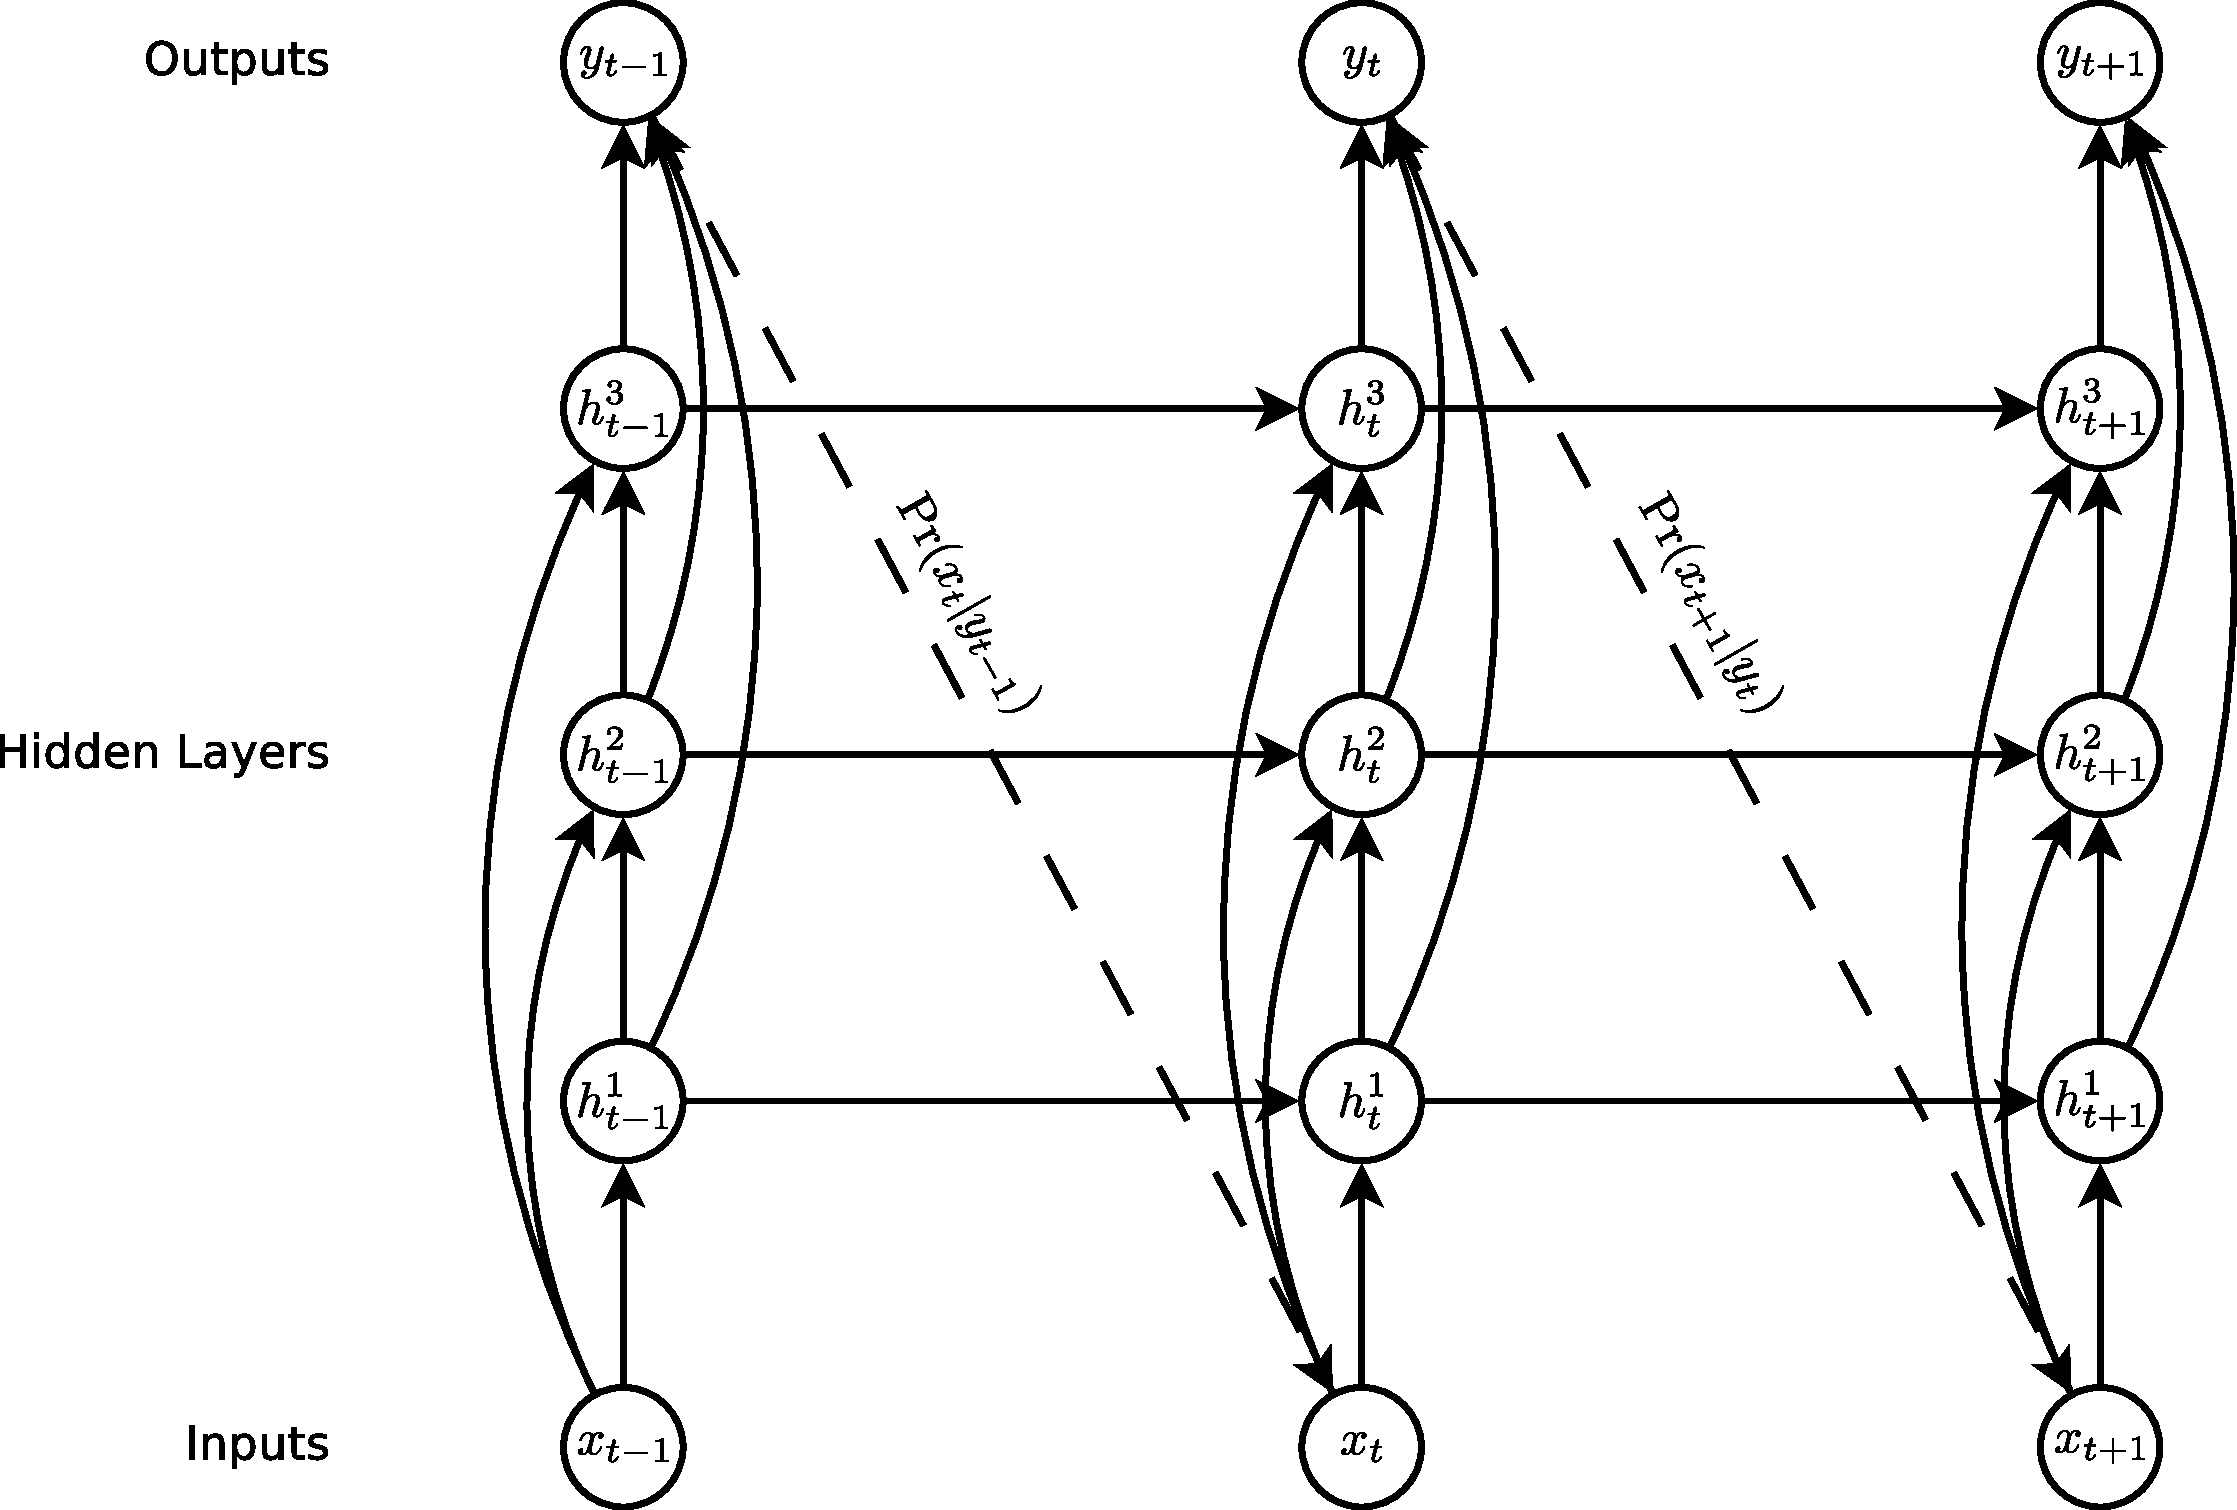
\includegraphics[scale = 0.3]{deep_predictor.pdf}
\caption{\textbf{Deep recurrent neural network prediction architecture.} The circles represent network layers, the solid lines represent weighted connections
and the dashed lines represent predictions. }
\flabel{deep_predictor}
\end{center}
\end{figure}

In \fref{deep_predictor}, an input vector sequence $\mathbf{x}=(x_1, \ldots, x_T)$ is passed long a weighted connections to a stack of $N$ recurrently interconnected hidden layers to compute the first hidden vector sequences $\mathbf{h}^n = (h^n_1,\ldots,h^n_T)$, and then the output vector sequence $\mathbf{y} = (y_1, \ldots, y_T)$

Each output vector $y_t$ is used to parameterise a predictive distribution $\Pr(x_{t+1}|y_t)$ over the possible next inputs $x_{t+1}$.

The first element $x_1$ of every input sequence is always a null vector whose entries are all zero; the network therefore emits a prediction for $x_2$, the first real input, with no prior information.
The network is `deep' in both space and time, in the sense that every piece of information passing either vertically or horizontally through the computation graph will be acted on by multiple successive weight matrices and nonlinearities.

How each hidden node is calculated can be shown in the following formula: 
\begin{align}
\label{eq:pred_hidden}
h^1_t &= \mathcal{H}\left(W_{i h^1} x_t + W_{h^{1}h^{1}} h^1_{t-1} + b_{h}^1 \right)\\
h^n_t &= \mathcal{H}\left(W_{i h^n} x_t + W_{h^{n-1}h^{n}} h^{n-1}_t + W_{h^{n}h^{n}} h^n_{t-1} + b_h^n \right)
\end{align} 
where the $W$ terms denote weight matrices (e.g.\ $W_{i h^n}$ is the weight matrix connecting the inputs to the $n^{th}$ hidden layer, $W_{h^{1}h^{1}}$ is the recurrent connection at the first hidden layer, and so on), the $b$ terms denote bias vectors (e.g.\ $b_o$ is output bias vector) and $\mathcal{H}$ is the hidden layer function. 

Given the hidden sequences, the output sequence can be calculated: 
\begin{align}
\label{eq:pred_output}
\hat{y}_t &= b_o + \sum_{n=1}^N{W_{h^n y} h^n_t}\\
y_t &= \mathcal{Y}(\hat{y}_t)	
\end{align}

The Long short-term memory (LSTM) network, developed by Hochreiter \& Schmidhuber in 1997, is an artificial neural net structure that unlike traditional RNNs doesn't have the vanishing gradient problem (compare the section on training algorithms below). It works even when there are long delays, and it can handle signals that have a mix of low and high frequency components. LSTM RNN outperformed other methods in numerous applications such as language learning and connected handwriting recognition.


That is how the network is built. 

In this project, the data are the sequence 

To enable the network to make prediction about a sequence, the output sequence is used as a parameter of the probability distribution $\Pr(x_{t+1}|y_t)$ of the next input. The form of distribution should be selected carefully to give high performing prediction. 

The probability given by the network to the input sequence x is
\begin{equation}
\Pr(\mathbf{x}) = \prod_{t=1}^T{\Pr(x_{t+1}|y_t)}
\end{equation}



\section{Experiments}
\subsection{Data collection}

As discussed in Section 3.1, the input to be translated to collected data is in video format and is processed by detecting pixel discrepancies between each frame. An example of detected pixel discrepancies is shown below where detected discrepancies between a frame range were highlighted to show accuracy in the construction of the letter ‘H.’ Note that the cursor does not interfere with detection due to disregard of pixels that have been accurately identified as pixels changed due to cursor for every iteration/frame.
%insert picture of 'detection data'
\begin{center}
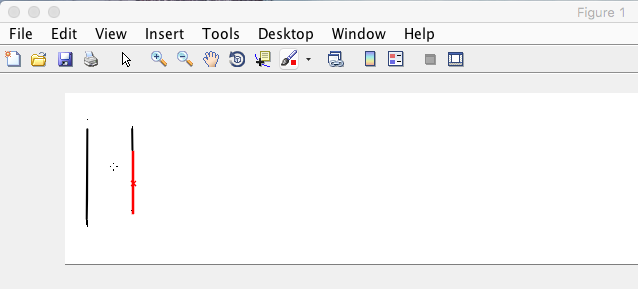
\includegraphics[scale = 0.4]{detection_data.png}
\end{center}

At the completion of the video processing there should be two accessible outputs for use later in software. The first is the last frame of the handwriting input and the second is the formatted data. Examples of these are shown below.
%insert picture of 'Hello World'
\begin{center}
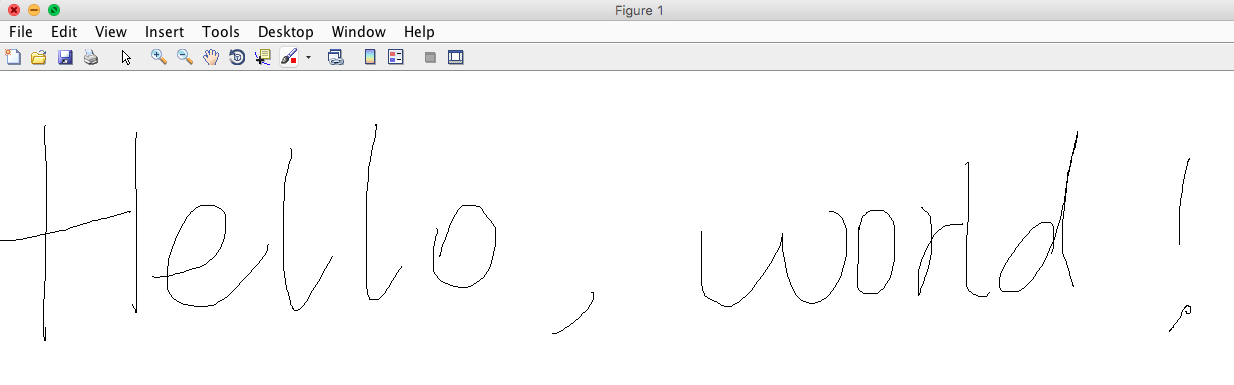
\includegraphics[scale = 0.2]{Hello_world.png}
\end{center}
%insert picture of 'Collected Data'
\begin{center}
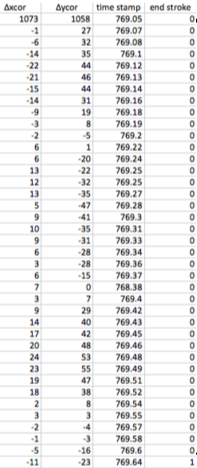
\includegraphics[scale = 0.7]{Collected_Data.png}
\end{center}


\subsection{Handwriting recognition}
\subsection{Handwriting generation}
(copying my presentation scripts)
The methods we will be using include handwriting recognition and Recurrent Neural Networks for sequence prediction. There are various languages involved. 



The workflow looks like this: 
First we collected trace of pen stroke using a tracking pad and screencast. Then we used the handwriting recognition technology to generate the contents of handwriting. With the data collected we trained a Recurrent Neural Network, which is later used for handwriting generation. 


After we collected and formatted the data, we use the data to train a recurrent neural network. The idea of RNN is to encode sequential correlation of ordered data points, in our case, the pen stroke data introduced earlier. The input and output variable will be the same sequence, excepted they are offsetted by one timestamp to make prediction possible. By training the recurrent neural network we are basically telling the program how to write. 


Instead of implementing the algorithms ourselves, we are using an off-the-shelf library we found online, rnnlib, which is written in C++. 


The architecture looks like this: 
The white dots are the input sequence, the black dots are the hidden layers, which are the essential part of any neural network architecture to store complex non-linear correlation. The grey dots are the output. 


The training of the network took longer time than we thought. Each epoch is taking 30 hours or so, and we only managed to run 7 epochs. So the network is not yet well trained. Nevertheless it’s giving us eligible results. Here are two examples: 


Hello, it’s me: 
I think it’s fair to say it’s doing its job. 
If we look carefully, we can see the ‘e’ at the end was not finished. That is because the end of stroke flag appeared too soon. The network predicted 


And I am your father.  
It is not so ideal, but at least we can tell the letters apart. 





\section{Conclusions}
Something about the power of rnn. Why it captures the patterns of penstroke. 

There are a few ways we can improve the project. 
To give the training a little more time
The rnn library we are using is not optimized for multiprocessors, or gpu, so we can improve on their code. 
We might also want to improve the architecture of the neural networks, and if that succeeds we will be famous. 




\subsubsection*{References}

\small{
[1] Alexander, J.A. \& Mozer, M.C. (1995) Template-based algorithms
for connectionist rule extraction. In G. Tesauro, D. S. Touretzky
and T.K. Leen (eds.), {\it Advances in Neural Information Processing
Systems 7}, pp. 609-616. Cambridge, MA: MIT Press.

[2] Bower, J.M. \& Beeman, D. (1995) {\it The Book of GENESIS: Exploring
Realistic Neural Models with the GEneral NEural SImulation System.}
New York: TELOS/Springer-Verlag.

[3] Hasselmo, M.E., Schnell, E. \& Barkai, E. (1995) Dynamics of learning
and recall at excitatory recurrent synapses and cholinergic modulation
in rat hippocampal region CA3. {\it Journal of Neuroscience}
{\bf 15}(7):5249-5262.
}

[4] Vincent, N., Seropian, A., Stamon, G.: Synthesis for handwriting
analysis. Pattern Recognit. Lett. 26(3), 267–275 (2005)



Below is not part of the report

\section{Submission of papers to NIPS 2015}

NIPS requires electronic submissions.  The electronic submission site is  
\begin{center}
   \url{http://papers.nips.cc}
\end{center}

Please read carefully the
instructions below, and follow them faithfully.
\subsection{Style}

Papers to be submitted to NIPS 2015 must be prepared according to the
instructions presented here. Papers may be only up to eight pages long,
including figures. Since 2009 an additional ninth page \textit{containing only
cited references} is allowed. Papers that exceed nine pages will not be
reviewed, or in any other way considered for presentation at the conference.
%This is a strict upper bound. 

Please note that this year we have introduced automatic line number generation
into the style file (for \LaTeXe and Word versions). This is to help reviewers
refer to specific lines of the paper when they make their comments. Please do
NOT refer to these line numbers in your paper as they will be removed from the
style file for the final version of accepted papers.

The margins in 2015 are the same as since 2007, which allow for $\approx 15\%$
more words in the paper compared to earlier years. We are also again using 
double-blind reviewing. Both of these require the use of new style files.

Authors are required to use the NIPS \LaTeX{} style files obtainable at the
NIPS website as indicated below. Please make sure you use the current files and
not previous versions. Tweaking the style files may be grounds for rejection.

%% \subsection{Double-blind reviewing}

%% This year we are doing double-blind reviewing: the reviewers will not know 
%% who the authors of the paper are. For submission, the NIPS style file will 
%% automatically anonymize the author list at the beginning of the paper.

%% Please write your paper in such a way to preserve anonymity. Refer to
%% previous work by the author(s) in the third person, rather than first
%% person. Do not provide Web links to supporting material at an identifiable
%% web site.

%%\subsection{Electronic submission}
%%
%% \textbf{THE SUBMISSION DEADLINE IS June 5, 2015. SUBMISSIONS MUST BE LOGGED BY
%% 23:00, June 5, 2015, UNIVERSAL TIME}

%% You must enter your submission in the electronic submission form available at
%% the NIPS website listed above. You will be asked to enter paper title, name of
%% all authors, keyword(s), and data about the contact
%% author (name, full address, telephone, fax, and email). You will need to
%% upload an electronic (postscript or pdf) version of your paper.

%% You can upload more than one version of your paper, until the
%% submission deadline. We strongly recommended uploading your paper in
%% advance of the deadline, so you can avoid last-minute server congestion.
%%
%% Note that your submission is only valid if you get an e-mail
%% confirmation from the server. If you do not get such an e-mail, please
%% try uploading again. 


\subsection{Retrieval of style files}

The style files for NIPS and other conference information are available on the World Wide Web at
\begin{center}
   \url{http://www.nips.cc/}
\end{center}
The file \verb+nips2015.pdf+ contains these 
instructions and illustrates the
various formatting requirements your NIPS paper must satisfy. \LaTeX{}
users can choose between two style files:
\verb+nips15submit_09.sty+ (to be used with \LaTeX{} version 2.09) and
\verb+nips15submit_e.sty+ (to be used with \LaTeX{}2e). The file
\verb+nips2015.tex+ may be used as a ``shell'' for writing your paper. All you
have to do is replace the author, title, abstract, and text of the paper with
your own. The file
\verb+nips2015.rtf+ is provided as a shell for MS Word users.

The formatting instructions contained in these style files are summarized in
sections \ref{gen_inst}, \ref{headings}, and \ref{others} below.

%% \subsection{Keywords for paper submission}
%% Your NIPS paper can be submitted with any of the following keywords (more than one keyword is possible for each paper):

%% \begin{verbatim}
%% Bioinformatics
%% Biological Vision
%% Brain Imaging and Brain Computer Interfacing
%% Clustering
%% Cognitive Science
%% Control and Reinforcement Learning
%% Dimensionality Reduction and Manifolds
%% Feature Selection
%% Gaussian Processes
%% Graphical Models
%% Hardware Technologies
%% Kernels
%% Learning Theory
%% Machine Vision
%% Margins and Boosting
%% Neural Networks
%% Neuroscience
%% Other Algorithms and Architectures
%% Other Applications
%% Semi-supervised Learning
%% Speech and Signal Processing
%% Text and Language Applications

%% \end{verbatim}

\section{General formatting instructions}
\label{gen_inst}

The text must be confined within a rectangle 5.5~inches (33~picas) wide and
9~inches (54~picas) long. The left margin is 1.5~inch (9~picas).
Use 10~point type with a vertical spacing of 11~points. Times New Roman is the
preferred typeface throughout. Paragraphs are separated by 1/2~line space,
with no indentation.

Paper title is 17~point, initial caps/lower case, bold, centered between
2~horizontal rules. Top rule is 4~points thick and bottom rule is 1~point
thick. Allow 1/4~inch space above and below title to rules. All pages should
start at 1~inch (6~picas) from the top of the page.

%The version of the paper submitted for review should have ``Anonymous Author(s)'' as the author of the paper.

For the final version, authors' names are
set in boldface, and each name is centered above the corresponding
address. The lead author's name is to be listed first (left-most), and
the co-authors' names (if different address) are set to follow. If
there is only one co-author, list both author and co-author side by side.

Please pay special attention to the instructions in section \ref{others}
regarding figures, tables, acknowledgments, and references.

\section{Headings: first level}
\label{headings}

First level headings are lower case (except for first word and proper nouns),
flush left, bold and in point size 12. One line space before the first level
heading and 1/2~line space after the first level heading.

\subsection{Headings: second level}

Second level headings are lower case (except for first word and proper nouns),
flush left, bold and in point size 10. One line space before the second level
heading and 1/2~line space after the second level heading.

\subsubsection{Headings: third level}

Third level headings are lower case (except for first word and proper nouns),
flush left, bold and in point size 10. One line space before the third level
heading and 1/2~line space after the third level heading.

\section{Citations, figures, tables, references}
\label{others}

These instructions apply to everyone, regardless of the formatter being used.

\subsection{Citations within the text}

Citations within the text should be numbered consecutively. The corresponding
number is to appear enclosed in square brackets, such as [1] or [2]-[5]. The
corresponding references are to be listed in the same order at the end of the
paper, in the \textbf{References} section. (Note: the standard
\textsc{Bib\TeX} style \texttt{unsrt} produces this.) As to the format of the
references themselves, any style is acceptable as long as it is used
consistently.

As submission is double blind, refer to your own published work in the 
third person. That is, use ``In the previous work of Jones et al.\ [4]'',
not ``In our previous work [4]''. If you cite your other papers that
are not widely available (e.g.\ a journal paper under review), use
anonymous author names in the citation, e.g.\ an author of the
form ``A.\ Anonymous''. 


\subsection{Footnotes}

Indicate footnotes with a number\footnote{Sample of the first footnote} in the
text. Place the footnotes at the bottom of the page on which they appear.
Precede the footnote with a horizontal rule of 2~inches
(12~picas).\footnote{Sample of the second footnote}

\subsection{Figures}

All artwork must be neat, clean, and legible. Lines should be dark
enough for purposes of reproduction; art work should not be
hand-drawn. The figure number and caption always appear after the
figure. Place one line space before the figure caption, and one line
space after the figure. The figure caption is lower case (except for
first word and proper nouns); figures are numbered consecutively.

Make sure the figure caption does not get separated from the figure.
Leave sufficient space to avoid splitting the figure and figure caption.

You may use color figures. 
However, it is best for the
figure captions and the paper body to make sense if the paper is printed
either in black/white or in color.
\begin{figure}[h]
\begin{center}
%\framebox[4.0in]{$\;$}
\fbox{\rule[-.5cm]{0cm}{4cm} \rule[-.5cm]{4cm}{0cm}}
\end{center}
\caption{Sample figure caption.}
\end{figure}

\subsection{Tables}

All tables must be centered, neat, clean and legible. Do not use hand-drawn
tables. The table number and title always appear before the table. See
Table~\ref{sample-table}.

Place one line space before the table title, one line space after the table
title, and one line space after the table. The table title must be lower case
(except for first word and proper nouns); tables are numbered consecutively.

\begin{table}[t]
\caption{Sample table title}
\label{sample-table}
\begin{center}
\begin{tabular}{ll}
\multicolumn{1}{c}{\bf PART}  &\multicolumn{1}{c}{\bf DESCRIPTION}
\\ \hline \\
Dendrite         &Input terminal \\
Axon             &Output terminal \\
Soma             &Cell body (contains cell nucleus) \\
\end{tabular}
\end{center}
\end{table}

\section{Final instructions}
Do not change any aspects of the formatting parameters in the style files.
In particular, do not modify the width or length of the rectangle the text
should fit into, and do not change font sizes (except perhaps in the
\textbf{References} section; see below). Please note that pages should be
numbered.

\section{Preparing PostScript or PDF files}

Please prepare PostScript or PDF files with paper size ``US Letter'', and
not, for example, ``A4''. The -t
letter option on dvips will produce US Letter files.

Fonts were the main cause of problems in the past years. Your PDF file must
only contain Type 1 or Embedded TrueType fonts. Here are a few instructions
to achieve this.

\begin{itemize}

\item You can check which fonts a PDF files uses.  In Acrobat Reader,
select the menu Files$>$Document Properties$>$Fonts and select Show All Fonts. You can
also use the program \verb+pdffonts+ which comes with \verb+xpdf+ and is
available out-of-the-box on most Linux machines.

\item The IEEE has recommendations for generating PDF files whose fonts
are also acceptable for NIPS. Please see
\url{http://www.emfield.org/icuwb2010/downloads/IEEE-PDF-SpecV32.pdf}

\item LaTeX users:

\begin{itemize}

\item Consider directly generating PDF files using \verb+pdflatex+
(especially if you are a MiKTeX user). 
PDF figures must be substituted for EPS figures, however.

\item Otherwise, please generate your PostScript and PDF files with the following commands:
\begin{verbatim} 
dvips mypaper.dvi -t letter -Ppdf -G0 -o mypaper.ps
ps2pdf mypaper.ps mypaper.pdf
\end{verbatim}

Check that the PDF files only contains Type 1 fonts. 
%For the final version, please send us both the Postscript file and
%the PDF file. 

\item xfig "patterned" shapes are implemented with 
bitmap fonts.  Use "solid" shapes instead. 
\item The \verb+\bbold+ package almost always uses bitmap
fonts.  You can try the equivalent AMS Fonts with command
\begin{verbatim}
\usepackage[psamsfonts]{amssymb}
\end{verbatim}
 or use the following workaround for reals, natural and complex: 
\begin{verbatim}
\newcommand{\RR}{I\!\!R} %real numbers
\newcommand{\Nat}{I\!\!N} %natural numbers 
\newcommand{\CC}{I\!\!\!\!C} %complex numbers
\end{verbatim}

\item Sometimes the problematic fonts are used in figures
included in LaTeX files. The ghostscript program \verb+eps2eps+ is the simplest
way to clean such figures. For black and white figures, slightly better
results can be achieved with program \verb+potrace+.
\end{itemize}
\item MSWord and Windows users (via PDF file):
\begin{itemize}
\item Install the Microsoft Save as PDF Office 2007 Add-in from
\url{http://www.microsoft.com/downloads/details.aspx?displaylang=en\&familyid=4d951911-3e7e-4ae6-b059-a2e79ed87041}
\item Select ``Save or Publish to PDF'' from the Office or File menu
\end{itemize}
\item MSWord and Mac OS X users (via PDF file):
\begin{itemize}
\item From the print menu, click the PDF drop-down box, and select ``Save
as PDF...''
\end{itemize}
\item MSWord and Windows users (via PS file):
\begin{itemize}
\item To create a new printer
on your computer, install the AdobePS printer driver and the Adobe Distiller PPD file from
\url{http://www.adobe.com/support/downloads/detail.jsp?ftpID=204} {\it Note:} You must reboot your PC after installing the
AdobePS driver for it to take effect.
\item To produce the ps file, select ``Print'' from the MS app, choose
the installed AdobePS printer, click on ``Properties'', click on ``Advanced.''
\item Set ``TrueType Font'' to be ``Download as Softfont''
\item Open the ``PostScript Options'' folder
\item Select ``PostScript Output Option'' to be ``Optimize for Portability''
\item Select ``TrueType Font Download Option'' to be ``Outline''
\item Select ``Send PostScript Error Handler'' to be ``No''
\item Click ``OK'' three times, print your file.
\item Now, use Adobe Acrobat Distiller or ps2pdf to create a PDF file from
the PS file. In Acrobat, check the option ``Embed all fonts'' if
applicable.
\end{itemize}

\end{itemize}
If your file contains Type 3 fonts or non embedded TrueType fonts, we will
ask you to fix it. 

\subsection{Margins in LaTeX}
 
Most of the margin problems come from figures positioned by hand using
\verb+\special+ or other commands. We suggest using the command
\verb+\includegraphics+
from the graphicx package. Always specify the figure width as a multiple of
the line width as in the example below using .eps graphics
\begin{verbatim}
   \usepackage[dvips]{graphicx} ... 
   \includegraphics[width=0.8\linewidth]{myfile.eps} 
\end{verbatim}
or % Apr 2009 addition
\begin{verbatim}
   \usepackage[pdftex]{graphicx} ... 
   \includegraphics[width=0.8\linewidth]{myfile.pdf} 
\end{verbatim}
for .pdf graphics. 
See section 4.4 in the graphics bundle documentation (\url{http://www.ctan.org/tex-archive/macros/latex/required/graphics/grfguide.ps}) 
 
A number of width problems arise when LaTeX cannot properly hyphenate a
line. Please give LaTeX hyphenation hints using the \verb+\-+ command.


\subsubsection*{Acknowledgments}

Use unnumbered third level headings for the acknowledgments. All
acknowledgments go at the end of the paper. Do not include 
acknowledgments in the anonymized submission, only in the 
final paper. 

\subsubsection*{References}

References follow the acknowledgments. Use unnumbered third level heading for
the references. Any choice of citation style is acceptable as long as you are
consistent. It is permissible to reduce the font size to `small' (9-point) 
when listing the references. {\bf Remember that this year you can use
a ninth page as long as it contains \emph{only} cited references.}

\small{
[1] Alexander, J.A. \& Mozer, M.C. (1995) Template-based algorithms
for connectionist rule extraction. In G. Tesauro, D. S. Touretzky
and T.K. Leen (eds.), {\it Advances in Neural Information Processing
Systems 7}, pp. 609-616. Cambridge, MA: MIT Press.

[2] Bower, J.M. \& Beeman, D. (1995) {\it The Book of GENESIS: Exploring
Realistic Neural Models with the GEneral NEural SImulation System.}
New York: TELOS/Springer-Verlag.

[3] Hasselmo, M.E., Schnell, E. \& Barkai, E. (1995) Dynamics of learning
and recall at excitatory recurrent synapses and cholinergic modulation
in rat hippocampal region CA3. {\it Journal of Neuroscience}
{\bf 15}(7):5249-5262.
}

\end{document}
